Una vez que se han entrenado y optimizado distintos modelos, se tiene
que identificar cuál de ellos consigue mejores resultados. Elegir un modelo u otro depende en cierta parte del objetivo del análisis y lo que se necesita extraer de él. Una manera para comparar los modelos es a través de las métricas de entrenamiento, validación y test. Estas métricas indican si el modelo es buen predictor, si está sobreajustado, y si cumple con los criterios de éxito propuestos.\\

Las métricas mas importantes se obtienen del análisis del conjunto de Test, ya que éste tiene las observaciones que no se utilizaron para armar el modelo, por lo que nos indica si es o no un buen predictor.\\

Esta comparación se detalla en la tabla \ref{tab:cuadro_comparativo-modelos} y la imagen \ref{fig:comparativo_modelos}. La comparación se realiza con todas las variantes que conjuntos de datos y modelos mencionadas en las secciones anteriores y está ordenada en función del Accuracy obtenido con el conjunto de test. Las métricas son de aquellos modelos generados con los hiperparámetros ya optimizados con Cross.Validation, y entrenados sin particiones utilizando todas las observaciones como train y ejecutado para predecir el conjunto de Test. Para una mayor claridad, se transcriben algunas definiciones:

\begin{itemize}
	\item DataSet-Completo: utiliza todas las variables disponibles.
	\begin{itemize}
		\item Modelos que se aplican sobre este dataset: SVMradial (SVM), rf (RandomForest), boosting (GradientBoosting), logistic (Regresión Logística), arbol (Arbol simple C5.0), LDA (LDA), KNN (KNN)  
	\end{itemize}
	\item DataSet-Alternativa1: utiliza las variables seleccionadas que por análisis de eliminación recursiva resultó tener mejores métricas y utilizando menos variables. \ref{analisis-var_importantes}.
		\begin{itemize}
		\item Modelos que se aplican sobre este dataset: RandomForest (RandomForest), Reg\_Logistica (Regresión Logística).
	\end{itemize}
	\item DataSet-Alternativa2: utiliza todas las variables disponibles excepto ``ciclo\_lectivo\_de\_cursada'' que resulta ser la mas influyente en los modelos generados que la incluyen. El análisis de variables relevante realizado con este conjunto de features \ref{analisis-var_importantes} demuestra que la mejor opción en cuestión de métricas es utilizar todas las variables.
			\begin{itemize}
		\item Modelos que se aplican sobre este dataset: RandomForest (RandomForest\_5), SVM\_5 (SVM), Reg\_Logistica\_5 (Regresión Logística), C50\_5 (Arbol simple C5.0), GradientBoosting\_5 (GradientBoosting).
	\end{itemize}
\end{itemize}

\begin{table}[!h]
	
	\caption{\label{tab:cuadro_comparativo-modelos}Resumen comparativo de algunos los modelos empleados}
	\centering
	\begin{tabular}[t]{cccc}
		\toprule
		\rowcolor{black}  \multicolumn{1}{c}{\textcolor{white}{\textbf{object}}} & \multicolumn{1}{c}{\textcolor{white}{\textbf{Test}}} & \multicolumn{1}{c}{\textcolor{white}{\textbf{Training}}} & \multicolumn{1}{c}{\textcolor{white}{\textbf{dataset}}}\\
		\midrule
		\rowcolor{gray!6}  SVMradial & 0.8420 & 0.8511 & DataSet-Completo\\
		RandomForest & 0.8405 & 0.9103 & DataSet-Alternativa1\\
		\rowcolor{gray!6}  rf & 0.8383 & 0.9200 & DataSet-Completo\\
		boosting & 0.8361 & 0.8740 & DataSet-Completo\\
		\rowcolor{gray!6}  logistic & 0.8354 & 0.8420 & DataSet-Completo\\
		\addlinespace
		Reg\_logistica & 0.8339 & 0.8345 & DataSet-Alternativa1\\
		\rowcolor{gray!6}  arbol & 0.8324 & 0.8552 & DataSet-Completo\\
		LDA & 0.8266 & 0.8301 & DataSet-Completo\\
		\rowcolor{gray!6}  KNN & 0.8039 & 0.8198 & DataSet-Completo\\
		RandomForest\_5 & 0.7849 & 0.9674 & DataSet-Alternativa2\\
		\addlinespace
		\rowcolor{gray!6}  SVM\_5 & 0.7820 & 0.7988 & DataSet-Alternativa2\\
		Reg\_logistica\_5 & 0.7717 & 0.7768 & DataSet-Alternativa2\\
		\rowcolor{gray!6}  C50\_5 & 0.7534 & 0.8147 & DataSet-Alternativa2\\
		GradienBoosting\_5 & 0.7520 & 0.7963 & DataSet-Alternativa2\\
		\bottomrule
	\end{tabular}
\end{table}


\begin{figure}[!htb]
	\centering
	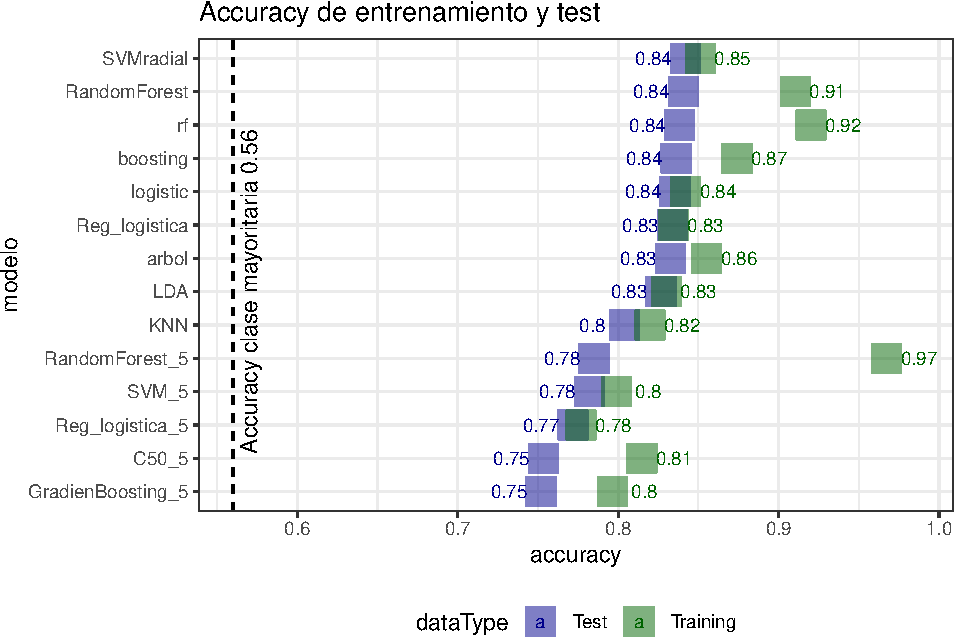
\includegraphics{imagenes/comparativo_modelos/unnamed-chunk-10-1.pdf}
	%\includegraphics[width=0.25\textwidth]{mesh}
	\caption{Accuracy de Entrenamiento y Test. Referencia Porcentaje de clase mayoritaria}
	\label{fig:comparativo_modelos}
\end{figure}


\subsubsection{Conclusión de comparación de Modelos}

En los modelos que se realizan con todas las variables(DataSet-Completo), podemos determinar
que el mejor modelo entrenado es el que emplea el método SVM. También
resulta ser el mejor cuando se elimina la variable que mas influencia
tiene en el resultado (DataSet-Alternativa2). De los métodos explicativos se puede decir que la
regresión logística seguido del árbol simple dan buenos resultados y no
muy alejado de las métricas de SVM.

Por otro lado, los distintos modelos de Random Forest dan muy buenos
resultados pero hay una diferencia muy grande en comparación a los otros
métodos entre train y test, por lo que hay riesgo de que hayan sufrido sobreajuste.

A su vez, se demostró que es factible utilizar menor cantidad de features y obtener resultados mejores utilizando el Método de RandomForest aunque la diferencia es mínima.

Por lo tanto, si lo importante es elegir un modelo que tenga mejor
capacidad predictiva, con estas combinaciones de datos, la mejor opción
es un SVM. No obstante, si se prioriza la interpretabilidad del modelo
para extraer conclusiones, se podría seleccionar el modelo Regresión
Logística o arbol simple.
Todos los modelos empleados superan ampliamente el nivel mínimo requerido que impone la clase mayoritaria que tiene el tablón con todas las observaciones. De esta manera, se demuestra que aún con algunas pocas variables referidas al desempeño académica o carrera académica, es posible identificar a posibles alumnos desertores.